\documentclass[UTF8]{article}
\usepackage[zihao=-4]{ctex} % ctex可以写中文，中括号里那句的意思是正文小四号
\usepackage[a4paper]{geometry} % 调整纸张大小和页边距的包，这里中括号中规定了纸张大小
\usepackage{array}
\usepackage{fancyhdr}
\usepackage{amsmath}
\usepackage{multirow}
\usepackage{tikz}
\geometry{left=2.5cm,right=2.5cm,top=2.5cm,bottom=2.5cm} % 页边距设置
\usepackage{caption}
\usepackage{wrapfig}
\usepackage{graphicx} % 用它在报告里加图
\usepackage{float}  
\usepackage{booktabs}   % 用于绘制专业的表格横线 
\usepackage{xcolor}    % 用于定义颜色
\usepackage{colortbl}  % 用于将颜色应用到表格行或单元格
\usepackage{makecell}  % 用于支持表头单元格内的换行

\pagestyle{fancy}
\rhead{迈克尔逊干涉仪}
\lhead{大学基础物理实验报告}
\cfoot{\thepage/7}
\rfoot{2026 年 5 月 15 日}

\begin{document}
	\thispagestyle{empty}
	\vspace*{0.5cm}
	
	\begin{figure}[h]
		\centering
		
\includegraphics[width=0.7\linewidth]{logo}
	\end{figure}
	\vspace*{0.1cm}
	\begin{center}
		\Huge{\textbf{大学基础物理实验报告}}\\
		\Huge{\textbf{《迈克尔逊干涉仪》}}
		
		\vspace*{0.1cm}
	\end{center}
	\begin{table}[h]
		\centering	
		\begin{Large}
			\begin{tabular}{p{3cm} p{5cm}<{\centering}}
				姓\qquad 名: & 陈秋实 \\
				\hline
				学\qquad 院: & 密码与网络空间安全学院 \\
				\hline
				学\qquad 号: & 2513318 \\
				\hline
				分\qquad 组: & L组1号 \\
				\hline
				实验时间: & 2026.5.15\\
				\hline
				
			\end{tabular}
		\end{Large}
	\end{table}
	\clearpage
	\normalsize
	\begin{center}
		\LARGE\textbf{迈克尔逊干涉仪}
	\end{center}
	
	\section{实验目的}
	\par 1.了解迈克尔孙干涉仪的结构原理并掌握调节方法。
	\par 2.观察等厚干涉、等倾干涉。
	\par 3.测量激光光源的波长。
	
	\section{实验器材}
	\par 迈克尔孙干涉仪，光源。
	\begin{figure}[!htbp]
		\centering
		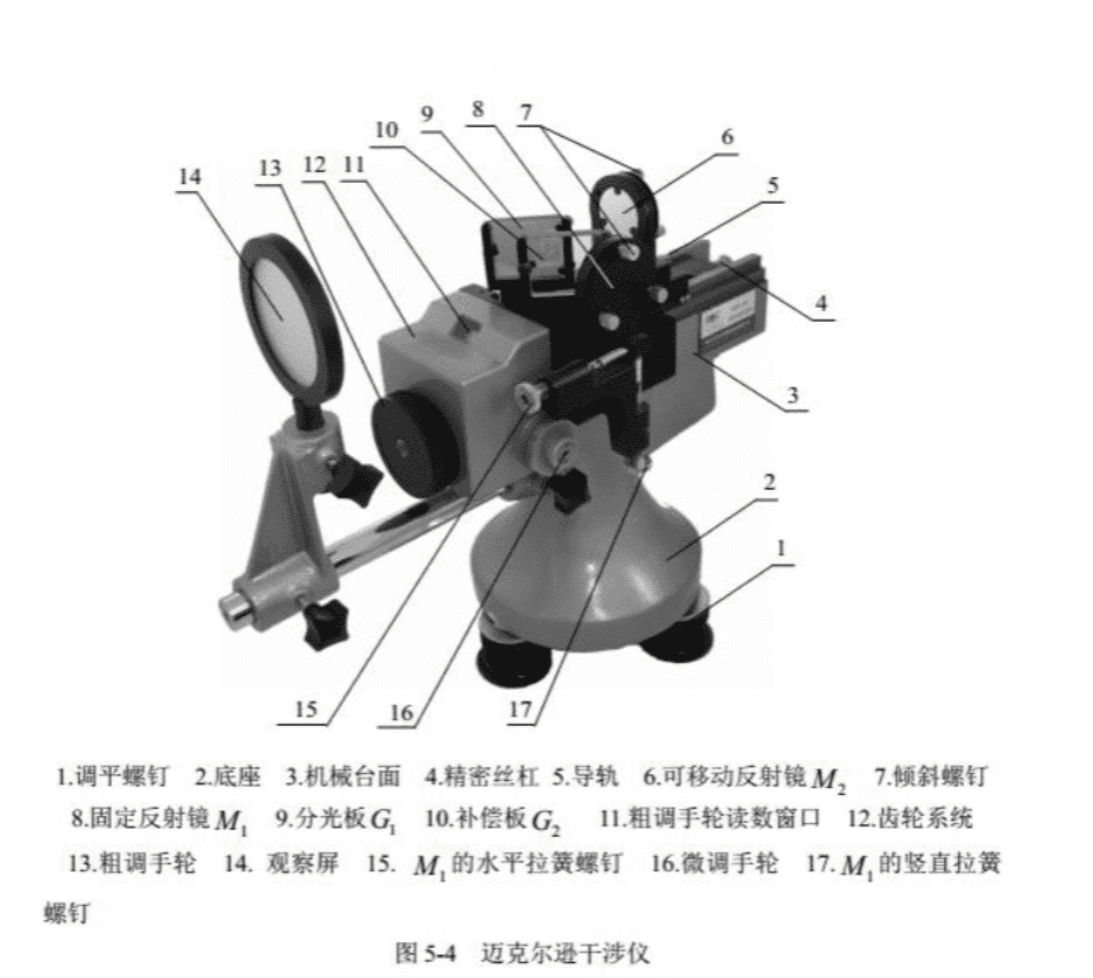
\includegraphics[width=1.0\textwidth]{干涉仪结构.png}
		
	\end{figure}
	
			\section{实验原理}

		\subsection{迈克尔逊干涉仪光路}
		如图1所示，从光源 $S$ 发出的一束光入射到分光板 $P_1$ 的后表面（半透半反膜）上，被分成两束光：反射光（1）和透射光（2）。反射光（1）垂直入射到平面反射镜 $M_1$ 上，经 $M_1$ 反射后再次透过 $P_1$ 到达观察位置 $E$；透射光（2）穿过补偿板 $P_2$ 后垂直入射到平面反射镜 $M_2$ 上，经 $M_2$ 反射后再次穿过 $P_2$，然后被 $P_1$ 的后表面反射到达 $E$。图中 $M_2'$ 是 $M_2$ 经 $P_1$ 后表面反射所成的虚像，因此两束光在 $E$ 处的干涉效果等效于 $M_1$ 与 $M_2'$ 之间的空气薄膜干涉。

		补偿板 $P_2$ 与分光板 $P_1$ 厚度、折射率均相同且平行放置，其作用是使两束光在玻璃中经过的光程相等，从而消除白光干涉时因色散导致的附加光程差。

		\begin{figure}[H]
			\centering
			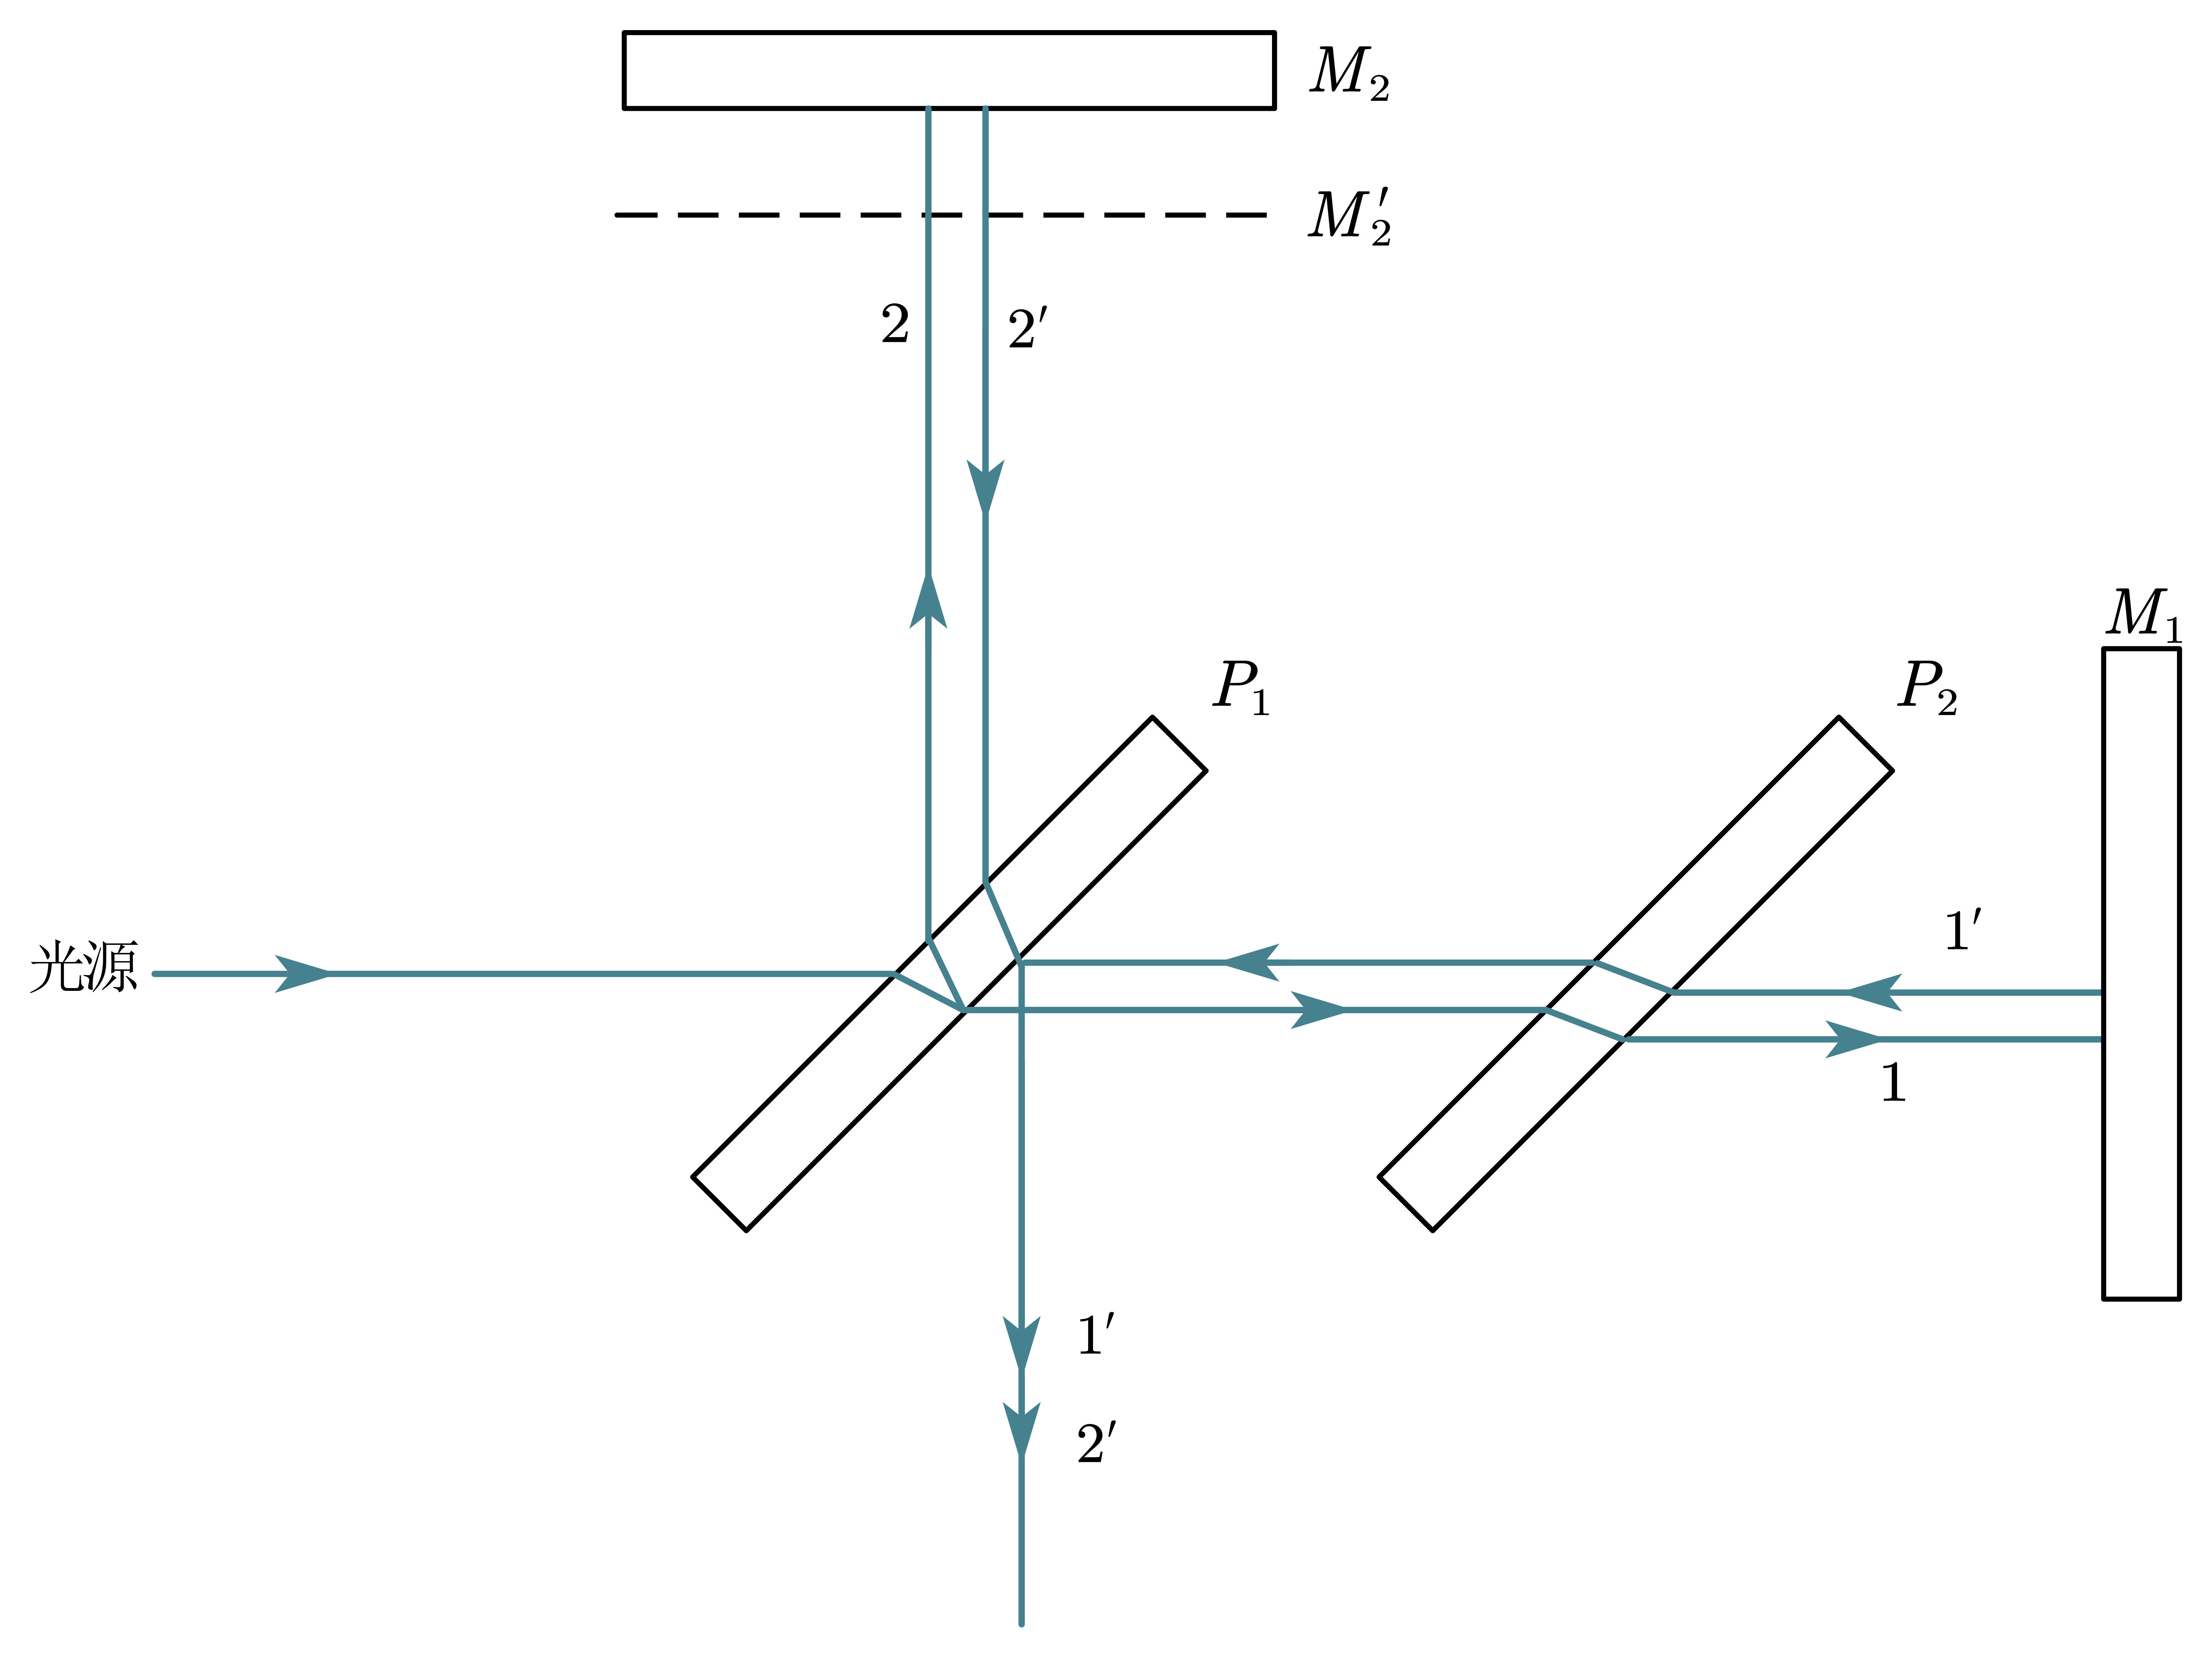
\includegraphics[width=0.5\textwidth]{迈克尔干涉仪原理.png}
			\caption{迈克尔孙干涉仪原理图}
		\end{figure}

		\subsection{等倾干涉}
		当 $M_1$ 与 $M_2$ 严格垂直时，$M_1$ 与 $M_2'$ 相互平行，形成厚度为 $d$ 的平行空气薄膜。对于入射角为 $\theta$ 的光线，两束反射光的光程差为
		\[
		\Delta = 2d\cos\theta
		\]
		相应的相位差为 $\delta = \frac{2\pi}{\lambda}\Delta$。当
		\[
		2d\cos\theta = k\lambda \quad (k = 0,1,2,\dots)
		\]
		时干涉加强，屏上呈现亮纹；当 $2d\cos\theta = (2k+1)\frac{\lambda}{2}$ 时干涉减弱，呈现暗纹。由于 $d$ 一定时，$\theta$ 相同的所有光线具有相同的光程差，因此形成的干涉条纹为同心圆环，称为等倾干涉条纹。

		在圆心处 $\theta = 0$，光程差最大：$\Delta = 2d$。当 $d$ 增大时，圆心处光程差增大，干涉级次 $k$ 升高，条纹从中心"冒出"并向远离中心方向移动；当 $d$ 减小时，条纹向中心"缩进"。每冒出或缩进一个条纹，对应光程差改变一个波长 $\lambda$，即 $d$ 改变了 $\lambda/2$。

		\subsection{等厚干涉}
		当 $M_1$ 与 $M_2$ 不完全垂直时，$M_1$ 与 $M_2'$ 之间形成劈尖形空气薄膜。当 $d$ 很小时，$\theta$ 变化对光程差的影响可以忽略，干涉条纹近似为平行于劈尖棱边的等间距直条纹，称为等厚干涉条纹。随着 $d$ 增大，条纹逐渐弯曲并向 $d$ 减小的方向凸出。

		\subsection{条纹移动数与 $d$ 变化量的关系}
		综合上述分析，无论等倾还是等厚干涉，每当 $d$ 改变 $\lambda/2$ 时，视场中某固定点处就有一个条纹移过。若条纹移动数为 $N$，则 $M_1$（或 $M_2$）移动的距离为
		\[
		\boxed{\delta d = N\frac{\lambda}{2}}
		\]
		由此式即可通过计数条纹移动数和测量 $d$ 的位移量来计算光源波长：
		\[
		\lambda = \frac{2\,\delta d}{N}
		\]

		\section{操作步骤}
	\subsubsection*{调节干涉仪，观察非定域干涉}
	\par \textbf{一、水平调节}\quad 调节干涉仪底脚螺丝，使仪器导轨平面水平，然后用锁紧圈锁住。
	\par \textbf{二、等臂调节}\quad 调节粗调手轮移动$M_2$镜，让$M_1,M_2$镜与分光板$G_1$,大致等距离。
	\par \textbf{三、最亮点重合}\quad 打开激光开关，检查激光输出嘴的位置和方向，让光束垂直射向$M_1$的中心部位。将观察屏转向一侧并周定，戴上墨镜，直接观察$M_2$镜，视野 中呈现两排分别由$M_1$、$M_2$反射回来的亮点，找准每排亮点中最亮的那个点，分别调 节$M_1$和$M_2$两个反射镜背后的调节螺华(先调$M_1$再调$M_2$),使两排亮点中最亮的 光点严格重合，此时说明$M_1$已垂直$M_2$。注意调节时调节螺丝的松紧要均衡，防止损坏调节螺丝。
	\par \textbf{四、条纹移到屏中央}\quad 将观察屏转回原位置，若上一步中的最亮点已经严格重合，则观察屏上可以观察到圆形干涉条纹，若没有条纹，可能是亮点没严格重合，或者条纹在屏幕边缘。调节粗调手轮使条纹大小、粗细适中，再轻微调节$M_1$,镜上的水平或竖直拉簧螺丝，使圆形条纹的中心位于屏中央。
	\par \textbf{五、观察非定域干涉}\quad 前后左右移动屏的位置和角度，发现干涉条纹的大小或形状发生变化，证明非定义域干涉是空间处处相干的。
	\par \textbf{六、条纹特征与$d$的关系} \quad 调节粗调手轮前后移动M2,观察条纹的“冒出”或“缩进”现象，判断M;与M之间的距离d是变大还是变小，并观察条纹的粗细、疏密和d之间的关系。
	
	\subsubsection*{测量激光波长}
	\par \textbf{一、仪器调零} \quad 因为旋转微调手轮时，粗调手轮随之变化，而旋转粗调手轮时
	微调手轮并不随之变化，所以测量前必须调零。方法如下：沿某方向（例如顺时针）
	将微调手轮调到零并记住旋转方向(为避免空程差，后面的测量都要沿此方向)，沿
	同一方向旋转粗调手轮使之对准某一刻度，注意此后粗调手轮不要再动。测量过
	程中若需要反方向旋转微调手轮，则一定要重新调零。
	\par \textbf{二、测量并计算波长} \quad 沿刚才的方向旋转微调手轮，条纹每冒出或缩进50个记录相应的M2的位置，连续记录6次以上，数据记录在表4-5-1中，用最小二乘法计算激光的波长。


	\section{数据处理}
	\begin{figure}[!htbp]
		\centering
		
\includegraphics[width=0.8\textwidth]{实验数据.jpg}
		\caption{实验数据记录(带签名)}
	\end{figure}
	
	
	\begin{table}[!htbp]
		\centering
		\begin{tabular}{|c|c|c|c|c|c|c|}
			\hline
			条纹移动数N1 & 0 & 50 & 100 & 150 & 200 & 250 \\
			\hline
			可移动镜位置d1/mm & 52.83751 & 52.85235 & 52.86820 & 52.88337 & 52.90152 & 52.91566 \\
			\hline
		\end{tabular}
		\caption{实验数据表格}
	\end{table}
	
	
	
	\begin{table}[!htbp]
		\centering
		\begin{tabular}{|c|c|c|c|c|c|}
			\hline
			$\Delta d/\mathrm{mm}$ & 0.01484 & 0.01585 & 0.01517 & 0.01815 & 0.01414  \\
			\hline
			波长 $\lambda/\mathrm{nm}$ & 593.6nm & 634.0nm & 606.8nm & 726.0nm & 565.6nm \\
			\hline
		\end{tabular}
		\caption{实验计算结果}
	\end{table}
	
	\subsubsection*{使用最小二乘法计算波长}
	\par 设条纹移动数 $N$ 与可移动镜位置 $d$ 满足线性关系：
		\[
		d = d_0 + \frac{\lambda}{2}N
		\]
		\par 对表中6组数据 $(N_i, d_i)$ 进行最小二乘线性拟合，设 $d = a + bN$，其中斜率 $b = \lambda/2$。由最小二乘公式：
		\[
		b = \frac{n\sum N_i d_i - \sum N_i \sum d_i}{n\sum N_i^2 - (\sum N_i)^2}
		\]
		\par 代入数据计算：
		\begin{align*}
		n &= 6,\quad \sum N_i = 750,\quad \sum N_i^2 = 1.375 \times 10^5 \\
		\sum d_i &= 317.25861\ \mathrm{mm},\quad \sum (N_i d_i) = 39671.162\ \mathrm{mm}
		\end{align*}
		\[
		b = \frac{6 \times 39671.162 - 750 \times 317.25861}{6 \times 1.375 \times 10^5 - 750^2} \approx 3.162 \times 10^{-4}\ \mathrm{mm}
		\]
		\[
		\lambda = 2b \approx 6.325 \times 10^{-4}\ \mathrm{mm} = 632.5\ \mathrm{nm}
		\]
		\par 与 He-Ne 激光器标准波长 632.8 nm 相比，相对误差约为 0.05\%。

		\subsubsection*{不确定度分析}
		\par \textbf{1. 最小二乘拟合的剩余标准差}
		\par 由残差 $r_i = d_i - (a + bN_i)$ 计算剩余标准差 $s$：
		\[
		s = \sqrt{\frac{\sum_{i=1}^{n} r_i^2}{n-2}} = 9.37 \times 10^{-4}\ \mathrm{mm}
		\]

		\par \textbf{2. 斜率 $b$ 的标准不确定度}
		\par 由最小二乘拟合理论，斜率 $b$ 的 A 类标准不确定度为
		\[
		s_b = \frac{s}{\sqrt{\sum (N_i - \bar{N})^2}} = \frac{9.37 \times 10^{-4}}{\sqrt{4.375 \times 10^4}} \approx 4.48 \times 10^{-6}\ \mathrm{mm}
		\]

		\par \textbf{3. 波长 $\lambda$ 的合成不确定度}
		\par 由 $\lambda = 2b$，波长的 A 类标准不确定度为
		\[
		u_A(\lambda) = 2s_b \approx 8.96 \times 10^{-6}\ \mathrm{mm} \approx 9.0\ \mathrm{nm}
		\]
		\par B 类不确定度主要来源于读数显微镜的仪器误差，其最小分度值为 \mbox{$10^{-4}$\,mm}，在测量范围内影响很小，此处忽略不计。合成标准不确定度近似为
		\[
		u_c(\lambda) \approx u_A(\lambda) = 9.0\ \mathrm{nm}
		\]
		\par 取包含因子 $k = 2$，扩展不确定度为
		\[
		U(\lambda) = k \cdot u_c(\lambda) \approx 18.0\ \mathrm{nm}
		\]

		\par \textbf{4. 最终结果}
		\[
		\boxed{\lambda = (632.5 \pm 18.0)\ \mathrm{nm} \quad (k = 2)}
		\]
		\par He-Ne 激光器标准波长 632.8 nm 落入本实验结果的置信区间内，表明测量结果在不确定度范围内与标准值一致。

	 \begin{figure}[!htbp]
	 	\centering
	 	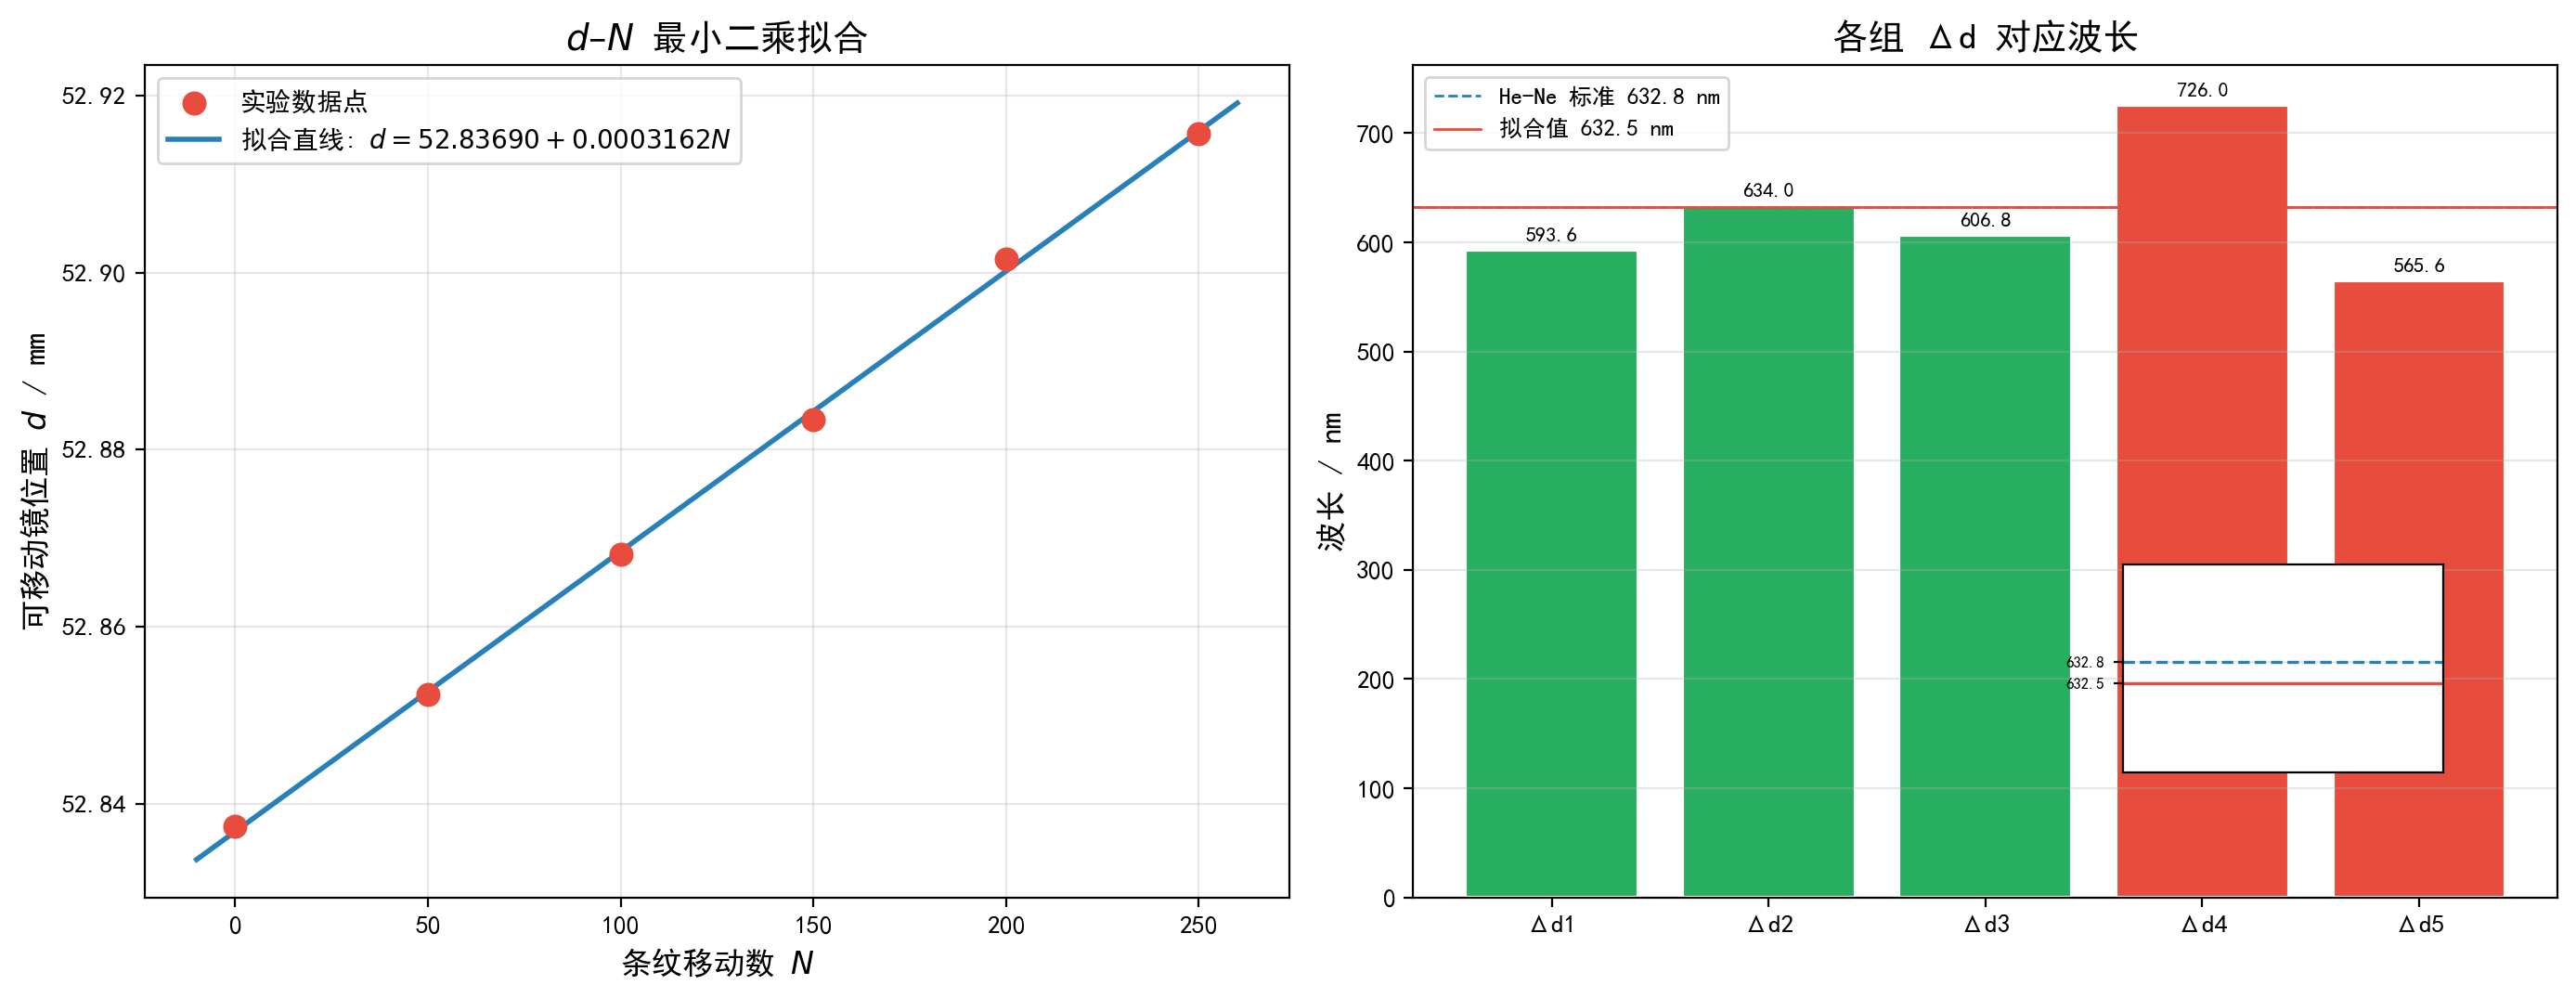
\includegraphics[width=1.0\textwidth]{迈克尔逊干涉仪_数据分析.png}
	 	\caption{数据分析可视化}
	 \end{figure}
	 
	 
	 \section{实验思考与总结}
	 \subsection*{操作要点}
	 调节最亮点重合是本实验最关键也是最耗时的步骤。先调 $M_1$ 再调 $M_2$，且调节螺丝松紧要均衡，否则极易导致两排光点始终错
	 位。仪器调零和始终沿同一方向旋转微调手轮是避免空程差的关键，一旦反向就必须重新调零。
	 
	 \subsection*{误差来源}
	 主要误差来源于条纹计数时人眼判断"冒出"或"缩进"的瞬间反应延迟，以及微调手轮读数的最小分度（$10^{-4}$\,mm）限制。从不确
	 定度分析来看，A 类不确定度（约 9\,nm）远大于 B 类，说明随机误差是主要限制因素。增大条纹计数间隔（如每 100
	 条记录一次）可部分改善。
	 
	 \subsection*{现象观察}
	 等倾干涉的同心圆环在 $d$ 增大时从中心"冒出"、减小时向中心"缩进"，与理论预测完全吻合。等厚干涉的直条纹在 $d$
	 增大时向劈尖薄端弯曲，直观体现了光程差随位置的变化。
	 
	 \subsection*{总结}
	 本实验测量得到 $\lambda = (632 \pm 18)\ \mathrm{nm}\ (k = 2)$，标准值 632.8\,nm 落在置信区间内，结果可信。通过动手调节
	 和观察，对分振幅干涉、等倾与等厚条纹特征、以及精密光学测量的系统误差控制有了直观深入的理解。
\end{document}